% Method overview: the gated cascade and the readiness ladder it assigns.
% Build: tectonic method-overview.tex   (standalone; include with \includegraphics)
\documentclass[tikz,border=4pt]{standalone}
\usepackage[T1]{fontenc}
\usepackage[scaled=0.92]{helvet}
\renewcommand{\familydefault}{\sfdefault}
\usepackage{amsmath,amssymb}
\usetikzlibrary{positioning,calc,arrows.meta,shapes.geometric,patterns}

% One hue per stage; each ladder rung takes the colour of the stage that decides it.
\definecolor{sZero}{HTML}{6B7A8F}
\definecolor{sOne}{HTML}{1B9E77}
\definecolor{sTwo}{HTML}{3A6FB0}
\definecolor{sThree}{HTML}{7B5EA7}
\definecolor{sFour}{HTML}{D9822B}
\definecolor{ink}{HTML}{25282E}
\definecolor{muted}{HTML}{7A808A}
\definecolor{paper}{HTML}{F4F5F7}

\tikzset{
  card/.style={draw=#1, line width=0.9pt, rounded corners=4pt, fill=#1!7,
    minimum width=3.12cm, minimum height=2.3cm},
  badge/.style={circle, fill=#1, text=white, font=\bfseries\small, minimum size=0.54cm, inner sep=0pt},
  title/.style={font=\bfseries\small, text=ink, anchor=west},
  q/.style={font=\scriptsize\itshape, text=muted, align=center, text width=2.75cm},
  chip/.style={rounded corners=1.6pt, fill=#1, text=white, font=\bfseries\tiny, inner xsep=2.5pt, inner ysep=1.4pt},
  flow/.style={-{Latex[length=2.2mm]}, line width=1.1pt, draw=ink!55},
  link/.style={-{Latex[length=1.9mm]}, line width=0.9pt, densely dotted, draw=#1!75, rounded corners=3pt},
}

\begin{document}
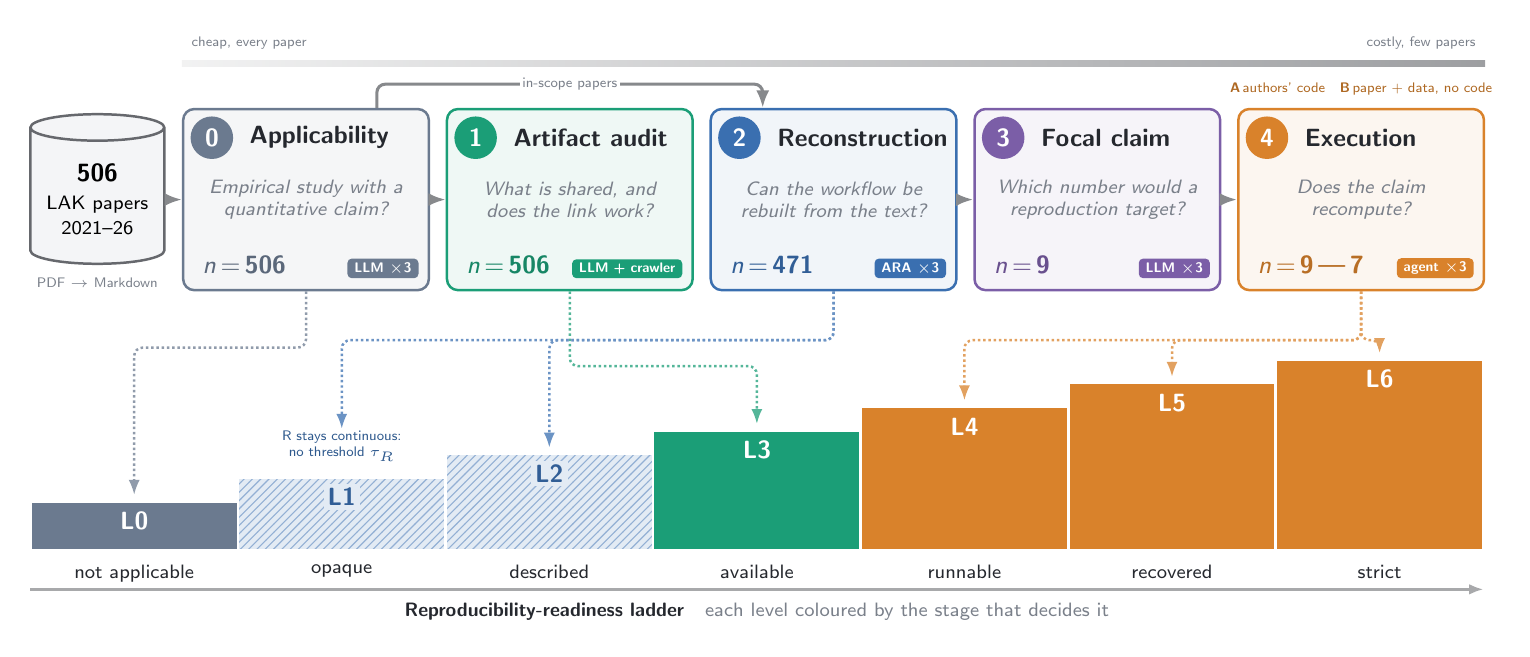
\begin{tikzpicture}[x=1cm,y=1cm]

%% ---------------------------------------------------------------- corpus
\node[cylinder, shape border rotate=90, aspect=0.22, draw=ink!70, fill=paper, line width=0.9pt,
      minimum width=1.7cm, minimum height=1.9cm, align=center, font=\small] (corpus) at (0,0)
      {\textbf{506}\\[-1pt]{\scriptsize LAK papers}\\[-2pt]{\scriptsize 2021--26}};
\node[font=\tiny, text=muted, below=1pt of corpus, align=center] {PDF $\rightarrow$ Markdown};

%% ---------------------------------------------------------------- stage cards
\def\gap{3.35}
\foreach \i/\col/\ttl/\qq/\n/\chiptxt in {
  0/sZero/Applicability/{Empirical study with a\\ quantitative claim?}/506/LLM $\times$3,
  1/sOne/Artifact audit/{What is shared, and\\ does the link work?}/506/LLM + crawler,
  2/sTwo/Reconstruction/{Can the workflow be\\ rebuilt from the text?}/471/ARA $\times$3,
  3/sThree/Focal claim/{Which number would a\\ reproduction target?}/9/LLM $\times$3,
  4/sFour/Execution/{Does the claim\\ recompute?}/9\,|\,7/agent $\times$3}
{
  \node[card=\col] (c\i) at ({2.65+\i*\gap},0) {};
  \node[badge=\col] (b\i) at ($(c\i.north west)+(0.38,-0.38)$) {\i};
  \node[title] at ($(b\i.east)+(0.08,0)$) {\ttl};
  \node[q] at ($(c\i.center)+(0,0.0)$) {\qq};
  \node[chip=\col, anchor=south east] at ($(c\i.south east)+(-0.14,0.16)$) {\chiptxt};
  \node[font=\small, text=\col!85!black, anchor=south west] at ($(c\i.south west)+(0.14,0.10)$)
       {\textit{n}\,=\,\textbf{\n}};
}
\draw[flow] (corpus.east) -- (c0.west);
\foreach \a/\b in {0/1,2/3,3/4} \draw[flow] (c\a.east) -- (c\b.west);
\draw[flow, rounded corners=3pt] ($(c0.north)+(0.9,0)$) -- ++(0,0.30) -| ($(c2.north)+(-0.9,0)$);

\node[font=\tiny, text=muted, fill=white, inner sep=1pt] at ($(c1.north)+(0,0.30)$) {in-scope papers};

\node[font=\tiny, text=sFour!80!black, anchor=south] at ($(c4.north)+(0,0.04)$)
     {\textbf{A}\,authors' code\quad\textbf{B}\,paper + data, no code};

% cost / depth gradient above the cascade
\shade[left color=ink!6, right color=ink!45]
      ($(c0.north west)+(0,0.52)$) rectangle ($(c4.north east)+(0,0.60)$);
\node[font=\tiny, text=muted, anchor=south west] at ($(c0.north west)+(0,0.62)$) {cheap, every paper};
\node[font=\tiny, text=muted, anchor=south east] at ($(c4.north east)+(0,0.62)$) {costly, few papers};

%% ---------------------------------------------------------------- readiness ladder
\def\xzero{-0.85}
\def\ybase{-4.45}
\def\stepw{2.636}
\def\steph{0.30}
\foreach \k/\col/\lab/\pat in {0/sZero/not applicable/0, 1/sTwo/opaque/1, 2/sTwo/described/1,
                               3/sOne/available/0, 4/sFour/runnable/0, 5/sFour/recovered/0, 6/sFour/strict/0}
{
  \pgfmathsetmacro{\h}{0.62+\k*\steph}
  \coordinate (r\k) at ({\xzero+\k*\stepw},\ybase);
  \coordinate (t\k) at ($(r\k)+(\stepw/2,\h)$);
  \ifnum\pat=1
    \path[fill=\col!14] (r\k) rectangle ++(\stepw,\h);
    \path[pattern=north east lines, pattern color=\col!55] (r\k) rectangle ++(\stepw,\h);
    \node[font=\bfseries\small, text=\col!85!black, fill=\col!14, inner sep=1.5pt] at ($(t\k)+(0,-0.25)$) {L\k};
  \else
    \path[fill=\col] (r\k) rectangle ++(\stepw,\h);
    \node[font=\bfseries\small, text=white] at ($(t\k)+(0,-0.25)$) {L\k};
  \fi
  \draw[white, line width=1pt] (r\k) rectangle ++(\stepw,\h);
  \node[font=\scriptsize, text=ink, below=2pt] at ($(r\k)+(\stepw/2,0)$) {\lab};
}
\node[font=\tiny, text=sTwo!80!black, align=center, anchor=south] at ($(t1)+(0,0.08)$)
     {R stays continuous:\\ no threshold $\tau_R$};
\draw[-{Latex[length=1.8mm]}, line width=0.9pt, draw=ink!40]
     ($(r0)+(0,-0.50)$) -- ($(r6)+(\stepw,-0.50)$)
     node[pos=0.5, below=1pt, font=\scriptsize, text=ink]
     {\textbf{Reproducibility-readiness ladder}\quad
      {\color{muted}each level coloured by the stage that decides it}};

%% ---------------------------------------------------------------- stage -> ladder links
\draw[link=sZero] (c0.south) |- ($(t0)+(0,1.95)$) -- ($(t0)+(0,0.08)$);
\draw[link=sOne]  (c1.south) -- ++(0,-0.95) -| ($(t3)+(0,0.08)$);
\draw[link=sTwo]  (c2.south) -- ++(0,-0.62) -| ($(t2)+(0,0.08)$);
\draw[link=sTwo]  (c2.south) -- ++(0,-0.62) -| ($(t1)+(0,0.62)$);
\draw[link=sFour] (c4.south) -- ++(0,-0.62) -| ($(t4)+(0,0.08)$);
\draw[link=sFour] (c4.south) -- ++(0,-0.62) -| ($(t5)+(0,0.08)$);
\draw[link=sFour] (c4.south) -- ++(0,-0.62) -| ($(t6)+(0,0.08)$);

\end{tikzpicture}
\end{document}
